
\documentclass{article}
\usepackage[utf8]{inputenc}
\usepackage{amsmath}

\usepackage{algorithm}
\usepackage{algorithmic}


\usepackage[english]{babel}
\usepackage[T1]{fontenc}
\usepackage{amsmath}
\usepackage{amsfonts}
\usepackage{amssymb}
\usepackage{csvsimple}





\usepackage{graphicx}


\newcommand{\vect}[1]{\ensuremath{\boldsymbol{\mathbf{#1}}}} 
\newcommand{\matr}[1]{\ensuremath{\boldsymbol{\mathbf{#1}}}}

\newcommand{\codevar}[1]{\textbf{#1}}



\usepackage{mathtools}
\DeclarePairedDelimiter\ceil{\lceil}{\rceil}
\DeclarePairedDelimiter\floor{\lfloor}{\rfloor}


\title{Exercise 3 - Spatial Statistics}
\author{Amir Ahmed}
\date{January 2020}


\begin{document}
	\maketitle
	
	\section*{Problem 1: Markov RF}
	Assume that we have observed seismic data over a domain $D \in \mathbb{R}^2$. We want to identify the underlying lithology distribution over D, the underlying lithology of a point is either sand or shale, $\lbrace 1, 0 \rbrace$ respectively.
	
	The observations have been collected on a regular $(75 \times 75)$ grid $L_d$, with seismic data being $\lbrace d(\vect x); \vect x \in L_d \rbrace$. Where $d(\vect x) \in \mathbb{R}$. 
	
	We have observed the lithology distribution in a geologically comparable domain $D_c \in \mathbb{R}^2$. Assume that this was collected on a regular $(66 \times 66)$ grid $L_{D_c}$. 
	
	We assume that the underlying lithology distribution can be represented by a Mosaic RF $\lbrace l(\vect x); \vect x \in  L_D\rbrace, l(\vect x) \in \lbrace 0, 1 \rbrace$.  
	
	
	\subsection*{Problem 1a)}
	 We start by looking at $L_d$.
	 Let the seismic data collection procedure follow the following likelihood model: 
	 $$\left[d_i | \vect l \right] = \begin{cases}
	 0.02 + U_i \text{ if sand, } l_i = 0 \\
	 0.08 + U_i \text{ if shale, } l_i = 1
	 \end{cases}$$
	 $i = 1, 2, \dots, n$. With $U_i$ being identically independently distributed $U_i \sim N(0, 0.06^2)$. This would make each observation point $d_i$ conditionally independent on $\vect l$. That will say: 
	\begin{equation}
		p(d_i | \vect l) = p(d_i | l_i) = \phi(d_i |\mu = 0.02 + 0.06l_i, \sigma^2 = 0.06^2)
	\end{equation}	
	 Where $\phi$ is the pdf of the normal distribution. As all observations are independent we thus have: 
	 \begin{equation}
	 	p(\vect d | \vect l) = \prod_{i=1}^{n}p(d_i | l_i) = \prod_{i=1}^{n}  \phi(d_i |\mu = 0.02 + 0.06l_i, \sigma^2 = 0.06^2)
	 \end{equation} 
	 
	 \begin{figure}[H]	
	 	\begin{center} 
	 		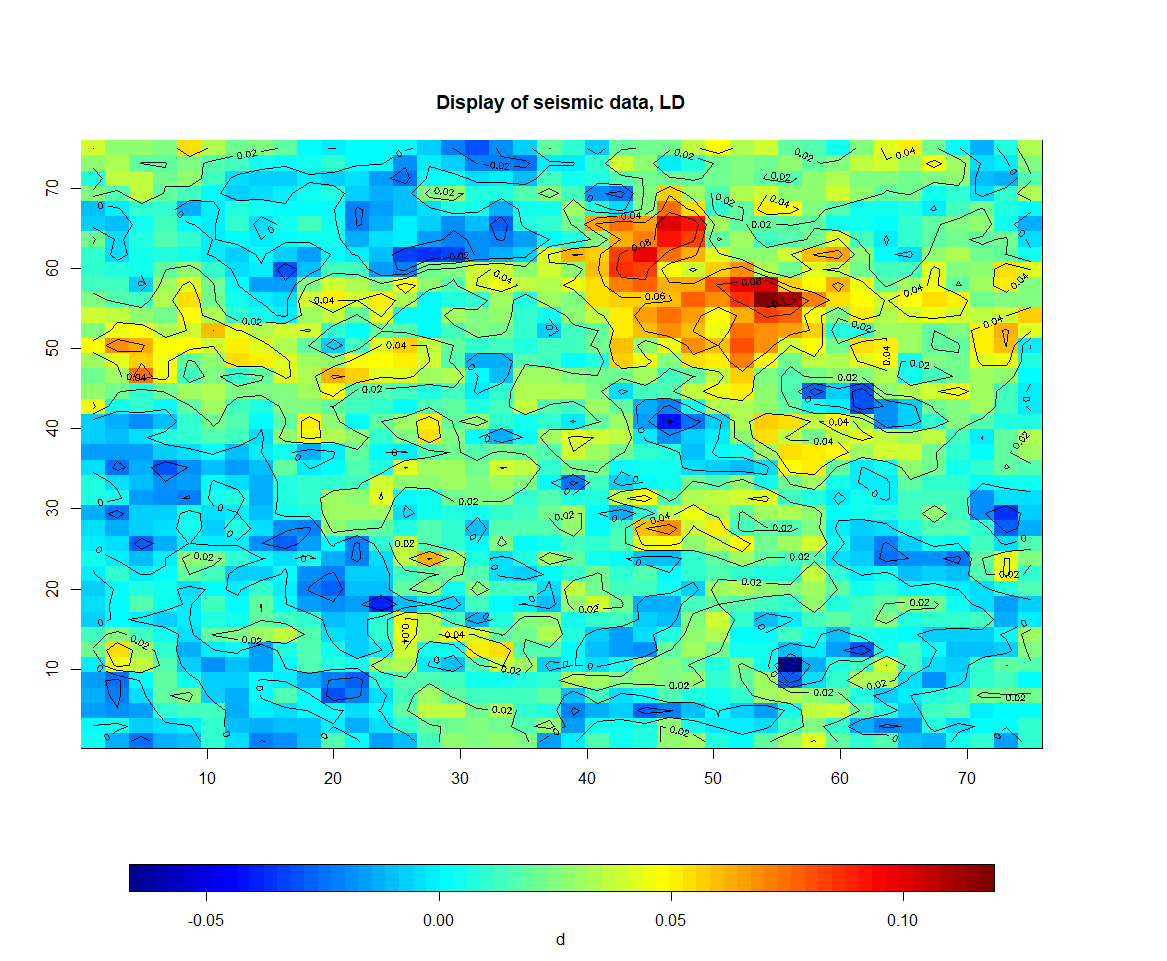
\includegraphics[scale=0.45]{figure1.png}
	 	\end{center}
	 	\caption{Display of seismic data $L_D$.}
	 	\label{fig:1a1} 
	\end{figure}
	 
	 
	 We display the observations from $L_D$ as a map in Figure \ref{fig:1a1}, there seems to be one large gathering where $d(\vect x)$ takes on relatively large values, there also seems to be some smaller gatherings of large $d(\vect x)$ in areas centered around the large one.  

	\newpage
	\subsection*{Problem 1b)}
\end{document}